\documentclass{article}

% ------------------------------------ %
%             Document Info            %
% ------------------------------------ %

\usepackage{../../../LaTeX-Preamables/Assign}

\begin{document}
\newcommand{\documentcourse}{MATH1853}
\newcommand{\documentnumber}{1}

% ------------------------------------ %
%                Header                %
% ------------------------------------ %

\begin{minipage}{0.07\textwidth}
    
\includegraphics[width=\linewidth]{../../../LaTeX-Preamables/LaTeX-Templates/HKULOGO256.png}
\end{minipage}
\hspace{0.02\textwidth}
\begin{minipage}{0.55\textwidth}
    \documentcourse

    Assignment \documentnumber

    SID: 3036268218
\end{minipage}
\begin{minipage}{0.35\textwidth}
    \begin{flushright}
        Jax

        \jobname.pdf

        \today
    \end{flushright}
\end{minipage}

\vspace{0.5cm}

\hrule

% ------------------------------------ %
%                Content               %
% ------------------------------------ %

Document prepared with LaTeX by myself. Solutions are my own.

\section*{Question 1}
Given $\lim_{x\to 0}(f+g)=2$ and $lim_{x\to 0}(2f-g)=-5$. We can find $lim_{x\to 0}(fg)$ by:
\begin{align*}
    \lim_{x\to 0}(f+g)                       & = 2                                       \\
    \lim_{x\to 0}(2f-g)                      & = -5                                      \\
    \lim_{x\to 0}(f+g) + \lim_{x\to 0}(2f-g) & = 2 + (-5)                                \\
    \lim_{x\to 0}(3f)                        & = -3                                      \\
    \lim_{x\to 0}(f)                         & = -1                                      \\
    \therefore \lim_{x\to 0}(g)              & = 2 - \lim_{x\to 0}(f)                    \\
                                             & = 3                                       \\
    \lim_{x\to 0}(fg)                        & = \lim_{x\to 0}(f) \cdot \lim_{x\to 0}(g) \\
                                             & = (-1) \cdot (3)                          \\
                                             & = -3
\end{align*}

\section*{Question 2}
\subsubsection*{Question 2a}
\begin{align*}
    \lim_{t\to 2}(\frac{2^{2t}+2^t-20}{2^t-4}) & = \lim_{t\to 2}\frac{(2^t-4)(2^t+5)}{2^t-4} \\
                                               & = \lim_{t\to 2}(2^t+5)                      \\
                                               & = 2^2+5                                     \\
                                               & = 9
\end{align*}
\subsubsection*{Question 2b}
\begin{align*}
    \lim_{x\to 0}(\tan(\frac{\pi}{4}\cos(\sin x^\frac{1}{3}))) & = \tan(\frac{\pi}{4}\cos(\sin 0^\frac{1}{3})) \\
                                                               & = \tan(\frac{\pi}{4}\cos(0))                  \\
                                                               & = 1
\end{align*}

\section*{Question 3}
To prove $\lim_{x\to 0^+}(\sqrt{x}\cdot (1 + \sin^2\frac{2\pi}{x}))=0$:
\begin{align*}
    -1 \leq \sin(\frac{1}{x}) \leq 1                                                                                  \\
    0 \leq \sin^2(\frac{1}{x}) \leq 1                                                                                 \\
    0 \leq \sin^2(\frac{2\pi}{x}) \leq 1                                                                              \\
    1 \leq (1+\sin^2(\frac{2\pi}{x})) \leq 2                                                                          \\
    \sqrt{x} \leq \sqrt{x}\cdot(1+\sin^2(\frac{2\pi}{x})) \leq 2\sqrt{x}                                              \\
    \lim_{x\to 0^+}\sqrt{x} \leq \lim_{x\to 0^+}\sqrt{x}\cdot(1+\sin^2(\frac{2\pi}{x})) \leq \lim_{x\to 0^+}2\sqrt{x} \\
    0 \leq \lim_{x\to 0^+}\sqrt{x}\cdot(1+\sin^2(\frac{2\pi}{x})) \leq 0                                              \\
    \therefore \lim_{x\to 0^+}\sqrt{x}\cdot(1+\sin^2(\frac{2\pi}{x})) = 0
\end{align*}

\section*{Question 4}
\subsubsection*{Question 4a}
We only need to consider the highest degree terms in the numerator and denominator, as x grows the highest degree terms would have the most effect on the limit:
\begin{align*}
    \lim_{x\to -\infty}(\frac{4x-3}{\sqrt{25x^2+4x}}) & = \lim_{x\to -\infty}(\frac{4x}{\sqrt{25x^2}}) \\
                                                      & = \lim_{x\to -\infty}(\frac{4x}{5|x|})         \\
                                                      & = (\frac{4\infty}{-5\infty})                   \\
                                                      & = -\frac{4}{5}                                 \\
\end{align*}

\subsubsection*{Question 4b}
Note: The limit of $\lim_{x\to \infty}(\frac{k}{x^n})$ for a constant $k$ must be $0$.
For this question, we must rationalize the numerator, because we can't combine the $x^2$ inside and outside the root:
\begin{align*}
    \lim_{x\to \infty}(\sqrt{4x^4+9x}-2x^2) & = \lim_{x\to \infty}(\sqrt{4x^4+9x}-2x^2)\cdot\frac{\sqrt{4x^4+9x}+2x^2}{\sqrt{4x^4+9x}+2x^2} \\
                                            & = \lim_{x\to \infty}(\frac{4x^4+9x-4x^4}{\sqrt{4x^4+9x}+2x^2})                                \\
                                            & = \lim_{x\to \infty}(\frac{9x}{\sqrt{4x^4+9x}+2x^2})                                          \\
                                            & = \lim_{x\to \infty}(\frac{\frac{9}{x}}{\sqrt{\frac{4x^4+9x}{x^4}}+2})                        \\
                                            & = \frac{\lim_{x\to \infty}\frac{9}{x}}{\lim_{x\to \infty}\sqrt{\frac{4x^4+9x}{x^4}}+2}        \\                                                                                     \\
                                            & = \frac{0}{\sqrt{4}+2}                                                                        \\
                                            & = 0                                                                                           \\
\end{align*}

\section*{Question 5}
To find the discontinuous points of $f(x)=\begin{cases}
        -x+5,        & \text{if } x\le -1          \\
        \sin(x^2-1), & \text{if } -1 \leq x \leq 1 \\
        \sqrt{x},    & \text{if } x > 1
    \end{cases}$:

A function $f(x)$ is \emph{discontinuous} at $x=a$ if: $\mathop {\lim }\limits_{x \to a} f( x) \ne f( a)$, or such that the limit does not exist.
\begin{align*}
    \lim_{x\to -1^-}(-x+5)                & = 6                                                                                                       \\
    \lim_{x\to -1^+}(\sin(x^2-1))         & = \sin(0) = 0                                                                                             \\
    \because \lim_{x\to -1^-}(-x+5)       & \neq \lim_{x\to -1^+}(\sin(x^2-1))                                                                        \\
    \therefore \text{Function has no limit at } x=-1                                                                                                  \\
    \lim_{x\to 1^-}(\sin(x^2-1))          & = \sin(0) = 0                                                                                             \\
    \lim_{x\to 1^+}(\sqrt{x})             & = \sqrt{1} = 1                                                                                            \\
    \because \lim_{x\to 1^-}(\sin(x^2-1)) & \neq \lim_{x\to 1^+}(\sqrt{x})                                                                            \\
                                          & \therefore \text{Function has no limit at } x= 1                                                          \\
                                          & \because \text{We know the function is continous on the left and right by their functions in the domain.} \\
                                          & \therefore \text{Function is discontinuous at } x=-1 \text{ and } x=1.
\end{align*}

\section*{Question 6}
Using the IVT to show that $\cos x=x$ has a solution in the interval $[0,1]$, we have to consider the roots of $f(x)=\cos x - x$:
\begin{align*}
    f(x) & = \cos x - x                                                                                                             \\
    f(0) & = \cos 0 - 0                                                                                                             \\
         & = 1                                                                                                                      \\
    f(1) & = \cos 1 - 1                                                                                                             \\
         & = 0.5403 - 1                                                                                                             \\
         & = -0.4597                                                                                                                \\
         & \because \text{0 lies in the interval } [f(0), f(1)]                                                                     \\
         & \therefore \text{By the IVT, there is a root in } [0,1]\text{, so there is a solution to } \cos x = x \text{ in } [0,1].
\end{align*}

\section*{Question 7}
\begin{minipage}{0.7\textwidth}
    Checking out the conditions of the function $f(x)$:
    \begin{enumerate}
        \item $\lim_{x\to -2}f(x)=1$
        \item $\lim_{x\to 1}f(x)=-\infty$
        \item $\lim_{x\to 2^-}f(x)=0$
        \item $\lim_{x\to 2^+}f(x)=2$
        \item $f(2)=1$
        \item $\lim_{x\to \infty}f(x)=1$
    \end{enumerate}
    Now we sketch the graph, labelling the axis, intercepts and asymptotes:
\end{minipage}
\begin{minipage}{0.3\textwidth}
    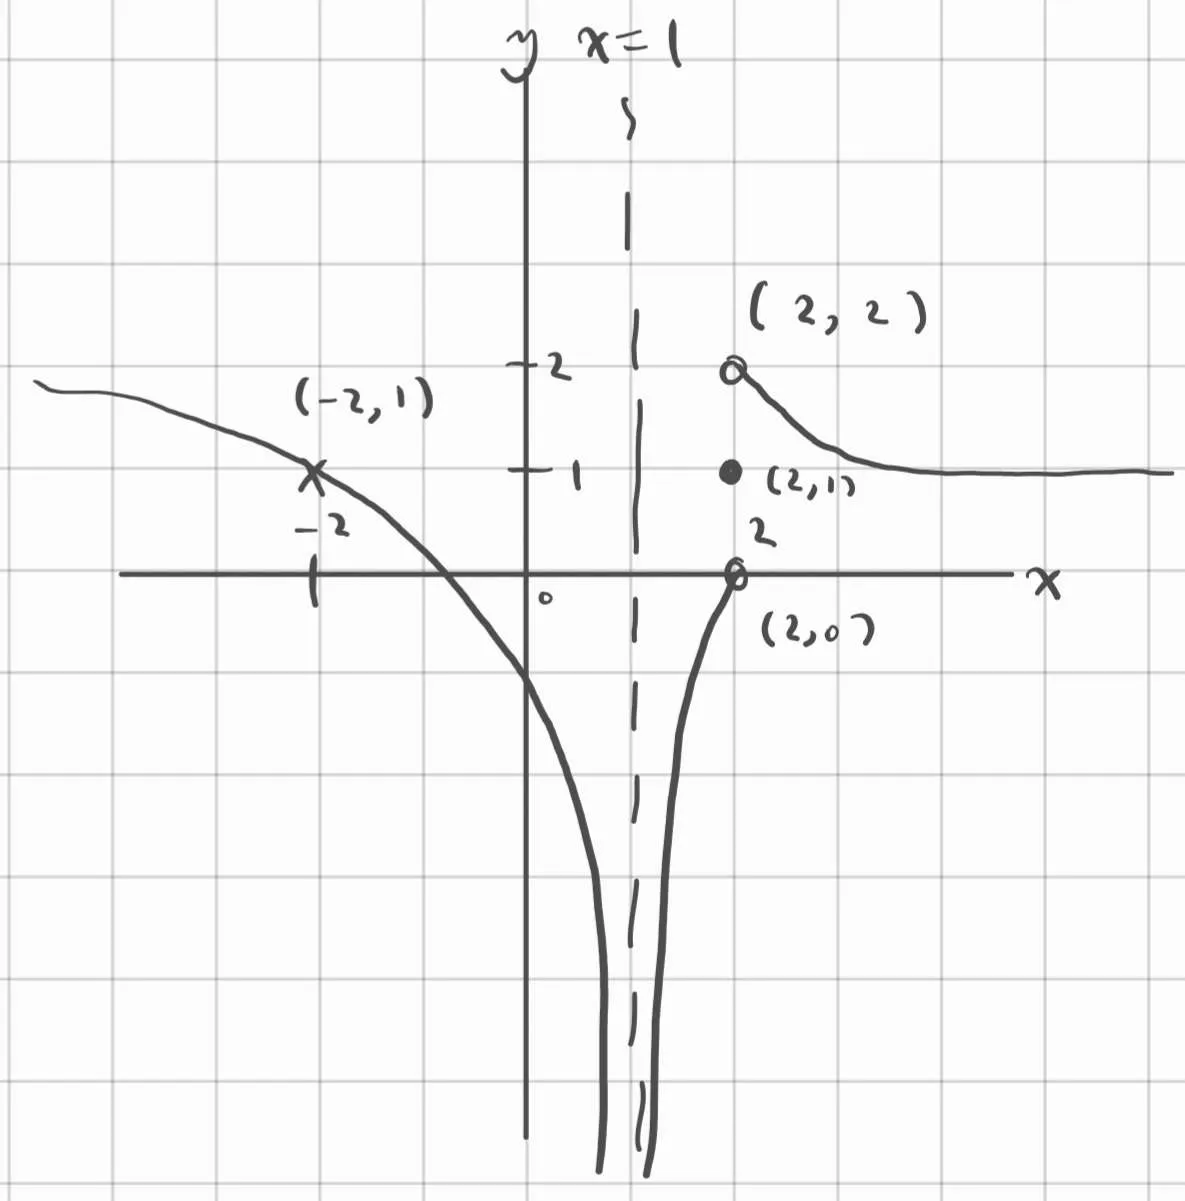
\includegraphics[width=\textwidth]{A1Q7.png}
\end{minipage}

\section*{Question 8}
Let $P(n)$ denote the perimeter of a regular $n$-gon inscribed in a unit circle.
\subsubsection*{Question 8a}
We know that the perimeter of a unit circle is $2\pi$. As the number of sides of the polygon increases, it gets closer and closer to being a circle as it's surface smooths out.  Hence, we can say that
$P(n)\to 2\pi$ as $n\to \infty$.
\subsubsection*{Question 8b}
We can find the unknown side of a triangle given the two sides and the angle between them using the cosine rule: $c=sqrt{a^2+b^2-2ab\cos C}$.

Consider the $n$ triangles inside a regular $n$-gon, with two of their sides from the center of the circle to the corners of the polygon. We then can make the following conclusions:
\begin{enumerate}
    \item $a,b$ = 1 as we are dealing with a unit circle.
    \item $C=\frac{2\pi}{n}$, as there are $n$ triangles.
\end{enumerate}
We then can write:
\begin{align*}
    P(n) & =n\sqrt{2-2\cos(\frac{2\pi}{n})}        \\
         & =n\sqrt{2-2(1-2\sin^2 (\frac{\pi}{n}))} \\
         & =n\sqrt{4\sin^2(\frac{\pi}{n})}         \\
         & =2n\sin(\frac{\pi}{n})
\end{align*}
\subsubsection*{Question 8c}
Question 8a shows us that $\lim_{x\to\infty}P(n)=2\pi$. Therefore:
\begin{align*}
    \lim_{n\to \infty}\frac{n}{\pi}\sin(\frac{\pi}{n}) & = \lim_{n\to \infty}\frac{2n\sin(\frac{\pi}{n})}{2\pi}    \\
                                                       & = \lim_{n\to \infty}\frac{P(n)}{2\pi}                     \\
                                                       & = \frac{\lim_{n\to \infty}P(n)}{\lim_{n\to \infty}2\pi}   \\
                                                       & = \frac{ \lim_{n\to \infty}2\pi}{ \lim_{n\to \infty}2\pi} \\
                                                       & = 1
\end{align*}
\subsubsection*{Question 8d}
Let $\theta=\frac{\pi}{n}$. The limit $n\to\infty$ is equivalent to $\theta\to 0$, as $\frac{\pi}{n}\to 0$ as $n\to \infty$. Therefore:
\begin{align*}
    \lim_{n\to \infty}\frac{n}{\pi}\sin(\frac{\pi}{n}) & = \lim_{\theta\to 0}\theta^{-1}\sin(\theta)   \\
                                                       & = \lim_{\theta\to 0}\frac{\sin\theta}{\theta}
\end{align*}
Therefore, we can say that $\lim_{\theta\to 0}\frac{\sin\theta}{\theta}=\lim_{n\to \infty}\frac{n}{\pi}\sin(\frac{\pi}{n})=1$.


\end{document}